
\begin{table*}
    \centering
    \begin{adjustbox}{max width=\textwidth}
        \begin{tabular}{|c|c|c|c|c|c|c|c|c|c|c|c|c|}
            \hline
            \multirow{3}{*}{Model}    &         & \multirow{2}{*}{Intent}   & Requested & Average        & Joint          &                &         & Average  & Joint    & \multirow{2}{*}{Response} &          \\
                                      & Domains & \multirow{2}{*}{Accuracy} & Slots     & Goal           & Goal           & Inform         & Success & Action   & Action   & \multirow{2}{*}{GLEU}     & Combined \\
                                      &         &                           & F1        & Accurracy      & Accuracy       &                &         & Accuracy & Accuracy &                           &          \\ \hline
            \multirow{3}{*}{\oursys~} & all     & 84.83                     & 95.53     & \textbf{72.38} & \textbf{48.44} & \textbf{73.08} & 62.19   & 58.32    & 46.31    & 20.04                     & 87.67    \\
                                      & seen    & 85.48                     & 95.88     & \textbf{74.23} & \textbf{52.05} & \textbf{74.72} & 63.85   & 60.19    & 48.69    & 24.66                     & 93.95    \\
                                      & unseen  & 84.45                     & 95.42     & \textbf{72.03} & \textbf{47.83} & \textbf{71.68} & 61.63   & 57.42    & 45.21    & 18.51                     & 85.16    \\ \hline
            {w/o}                     & all     & 75.08                     & 92.80     & 62.47          & 39.52          & 48.13          & 44.27   & 40.38    & 30.71    & 11.41                     & 57.61    \\
            {Two Step}                & seen    & 75.75                     & 93.13     & 64.66          & 42.76          & 50.26          & 46.47   & 41.96    & 32.42    & 13.75                     & 62.11    \\
            {Training}                & unseen  & 75.79                     & 92.90     & 62.60          & 39.25          & 47.55          & 44.32   & 40.25    & 30.66    & 11.03                     & 56.97    \\ \hline
            {w/o}                     & all     & 83.14                     & 94.67     & 64.70          & 38.47          & 59.88          & 53.88   & 54.14    & 43.07    & 21.15                     & 78.03    \\
            {Domain}                  & seen    & 84.34                     & 95.10     & 67.62          & 43.39          & 62.30          & 56.64   & 56.61    & 45.92    & 27.10                     & 86.57    \\
            {Schema}                  & unseen  & 82.96                     & 94.52     & 63.95          & 37.59          & 58.65          & 53.25   & 53.22    & 42.20    & 19.33                     & 75.28    \\ \hline
            % {w/o}                  & all     & 88.22                     & 95.72     & 71.51          & 42.68          & 64.15          & 60.98   & 57.34    & 45.26    & 20.70                     & 83.27    \\
            % {User}                 & seen    & 89.02                     & 96.07     & 73.86          & 47.02          & 65.80          & 63.17   & 59.48    & 47.83    & 25.96                     & 90.44    \\
            % {Actions}              & unseen  & 87.94                     & 95.59     & 71.05          & 41.78          & 63.09          & 60.73   & 56.46    & 44.41    & 18.82                     & 80.73    \\ \hline
            {w/o}                     & all     & 87.50                     & 95.48     & 71.54          & 43.20          & 50.96          & 56.89   & 53.67    & 41.73    & 17.62                     & 71.54    \\
            {DB}                      & seen    & 88.26                     & 95.85     & 73.87          & 47.62          & 53.03          & 59.08   & 55.73    & 43.91    & 23.12                     & 79.17    \\
            {Results}                 & unseen  & 87.19                     & 95.36     & 71.04          & 42.17          & 50.33          & 56.95   & 53.17    & 41.52    & 16.07                     & 69.70    \\ \hline
            {w/o Sys}                 & all     & 87.56                     & 96.00     & 72.86          & 44.52          & 60.13          & 61.91   & 57.98    & 45.86    & 21.02                     & 82.04    \\
            {Action}                  & seen    & 88.25                     & 96.32     & 75.11          & 48.77          & 61.69          & 64.04   & 60.12    & 48.37    & 26.56                     & 89.43    \\
            {Names}                   & unseen  & 87.38                     & 95.91     & 72.44          & 43.60          & 59.61          & 61.75   & 57.29    & 45.26    & 19.16                     & 79.84    \\ \hline
        \end{tabular}
    \end{adjustbox}
    \caption{Ablation Study of~\oursys.}
    \label{tab:ablation-results}
\end{table*}

\section{Results}
\begin{table}
    \begin{adjustbox}{max width=0.45\textwidth}
        \begin{tabular}{|c|c|c|c|c|}
            \hline
            \multirow{2}{*}{Model} & Intent   & Requested & Average & Joint \\
                                   & Accuracy & Slot F1   & GA      & GA    \\ \hline
            SGD Baseline           & 90.60    & 96.50     & 56      & 25.40 \\ \hline
            FastSGT                & 90.33    & 96.33     & 60.66   & 29.20 \\ \hline
            Seq2Seq-DU             & 91.00    & -         & -       & 30.10 \\ \hline
            DSGFNET                & -        & -         & -       & 32.10 \\ \hline
            \oursys~               & 81.49    & 95.97     & 74.08   & 49.73 \\ \hline
        \end{tabular}
    \end{adjustbox}
    \caption{Results on SGD test set. Our approach significantly outperforms baselines methods in terms of average and joint goal accuracy.}
    \label{tab:other-results}
\end{table}

Since there are no End-to-End TOD systems for the SGD dataset, we re-implemented some of the popular baseline methods to
compare with our approach and present the results in Table~\ref{tab:main-results}.

We can see that~\oursys~outperforms all the baselines across all metrics except GLEU. An explanation of this could be that since we
replaced the dialog history with the dialog state, the model lost a lot of exposure to dialog utterances.
Another reason could be that, while the system response requires a fluent generation, all other parts of the generation can be deemed as a structured generation.
A greedy decoding strategy generally works well for structured generation, but is not the best strategy for fluent generation, whereas
nucleus and top-k sampling strategies are better suited for fluent generation, but are not the best for structured generation.
We formulated the problem as a single sequence generation, and we can only select one strategy, so there is bound to be a trade-off since
there is no one strategy that is best suited for both fluent and structured generation.
We opted to use greedy decoding, which may have been the cause for the loss of fluency in the response generation.

We evaluate the DST performance of~\oursys~with the evaluation script provided by the SGD dataset and present our results alongside
other baseline DST models in Table~\ref{tab:other-results}.
We can see that even though our method is not specifically designed for DST, still it significantly outperforms the baselines models in the
important metrics: Average and Joint Goal Accuracy.

\subsection{Long Range Dialog Dependencies}

\begin{figure}[t]
    \centering
    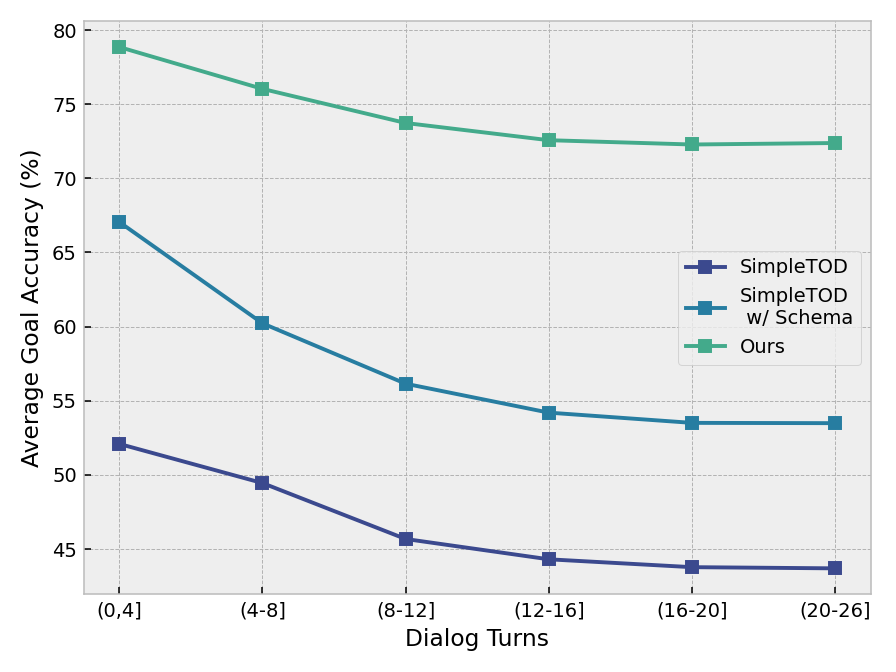
\includegraphics[width=\linewidth]{assets/dialog_turns.png}
    \caption{
        Performance of dialog systems on the SGD test set with respect to dialog turns
    }
    \label{fig:dialog_turns}
\end{figure}

In order to process dialogs that have a large number of turns, a system must be effective at capturing long range dependencies.
To test this ability, we group the test dialogs based on the number of turns and evaluate the performance of~\oursys~and a few baseline systems on each group.
As shown in Figure~\ref{fig:dialog_turns},~\oursys~outperforms the baseline systems across all groups.

Generally, in the first few turns of a dialog, the main focus is on figuring out what the user wants. The user could switch before mulitple options before finally deciding on one, however
towards the end of a dialog, usually the user has a clear idea of what they want, so he or she is less likely to make many changes.
For the first few turns, we have observed that there is a steeper drop in performance of the baseline when compared to~\oursys~.
A possible explanation of this could be that, since we pass the dialog summary to the model, it contains the correct state of the dialog at the previous turn, which helps the model to make better predictions.
Whereas in the baseline system, the model has to infer the previous state from the dialog history, which is a more difficult task.
In groups with large number of turns, both the baseline and~\oursys~perform similarly, which suggests even though~\oursys~does well in capturing
medium range dependencies, long range dependencies are still a challenge for the model.


\subsection{Two Step Training}

\begin{figure}[t]
    \centering
    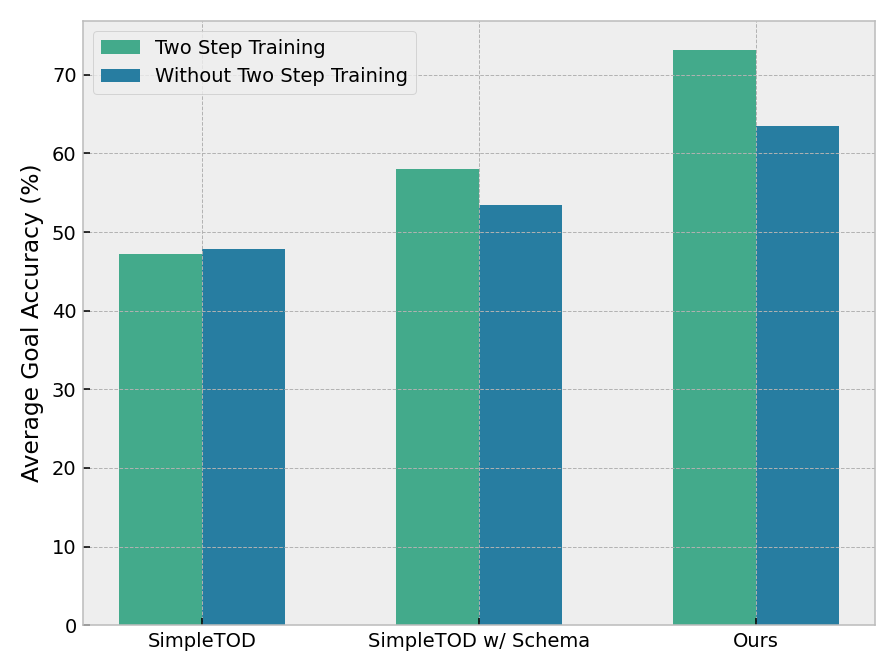
\includegraphics[width=\linewidth]{assets/two_step_training.png}
    \caption{
        Effect of Two Step Training on dialog systems
    }
    \label{fig:two_step_training}
\end{figure}

To better understand the effect of the two step training process, we compared~\oursys~and a few baseline systems with and without the two step training process.
In Figure~\ref{fig:two_step_training}, we can see that models that incorporate schema benefit from the two step training process.
\textbf{I am unable to come up with a solid explanation for why this happens, maybe you can think of something.}

\subsection{Ablation Study}

To get a better understanding of the different components of our model, we drop a certain component of~\oursys~to show effect on the performance
and report an ablation study in Table~\ref{tab:ablation-results}.
We can see that dropping two step training drastically degrades performance across all metrics, which suggests the importance of the training mechanism for~\oursys.

The role of schema is also important as we can see that the performance of~\oursys~drops across all metrics when we drop schema.
Another important aspect to notice here is that this variant has the largest difference in performance between seen and unseen domains.
These observations indicate that schema not only aids the model to generalize to new domains, but also plays a central role in the overall performance of the system.

\textbf{Write this section after experiments finish}We can observe that removing database results has a large impact on the metrics related to system actions.
We can see that removing list of system actions has decreased the metrics related to system actions, particularly Inform.
However, there is no significant decrease in metrics related to DST and system response. Database results have some correlation with DST,
so these components have a larger effect on DST when compared to list of system actions. As expected, the major drop in performance occurs when we
elect to drop schema. Not only does the performance drops significantly in the unseen domain, there is also a performance degradation
across all other metrics by a noticeable amount. This shows that schema is an important component in our approach as
it not only helps the model to generalize to new domains, but also plays a crucial role in the overall performance of the system.






\subsection{SGD-X}
% \begin{table*}
%     \centering
%     \begin{adjustbox}{max width=\textwidth}
%         \begin{tabular}{|c|c|c|c|c|c|c|c|c|c|c|c|c|}
%             \hline
%             \multirow{3}{*}{Model} & \multirow{2}{*}{Intent}   & Requested   & Average     & Joint       &            &             & Average     & Joint       & \multirow{2}{*}{Response} &              \\
%                                    & \multirow{2}{*}{Accuracy} & Slots       & Goal        & Goal        & Inform     & Success     & Action      & Action      & \multirow{2}{*}{GLEU}     & Combined     \\
%                                    &                           & F1          & Accurracy   & Accuracy    &            &             & Accuracy    & Accuracy    &                           &              \\ \hline
%             \oursys~               & 55.63, 7.7                & 89.67, 0.29 & 50.23, 3.84 & 29.46, 1.31 & 38.90, 2.9 & 26.47, 2.62 & 38.03, 2.12 & 33.60, 1.37 & 15.60, 0.91               & 48.29, 3.53  \\ \hline
%             SimpleTod w/ Schema    & 23.37, 6.03               & 88.23, 1.42 & 19.99, 4.29 & 10.75, 2.89 & 28.76, 7.7 & 16.21, 6.79 & 28.21, 5.2  & 24.19, 4.4  & 14.14, 3.39               & 36.62, 10.14 \\ \hline
%         \end{tabular}
%     \end{adjustbox}
%     \caption{SGD-x results on unseen domain. The mean and standard deviation across all 5 versions is reported for each metric}
%     \label{tab:sgdx-results}
% \end{table*}



\begin{figure}[t]
    \centering
    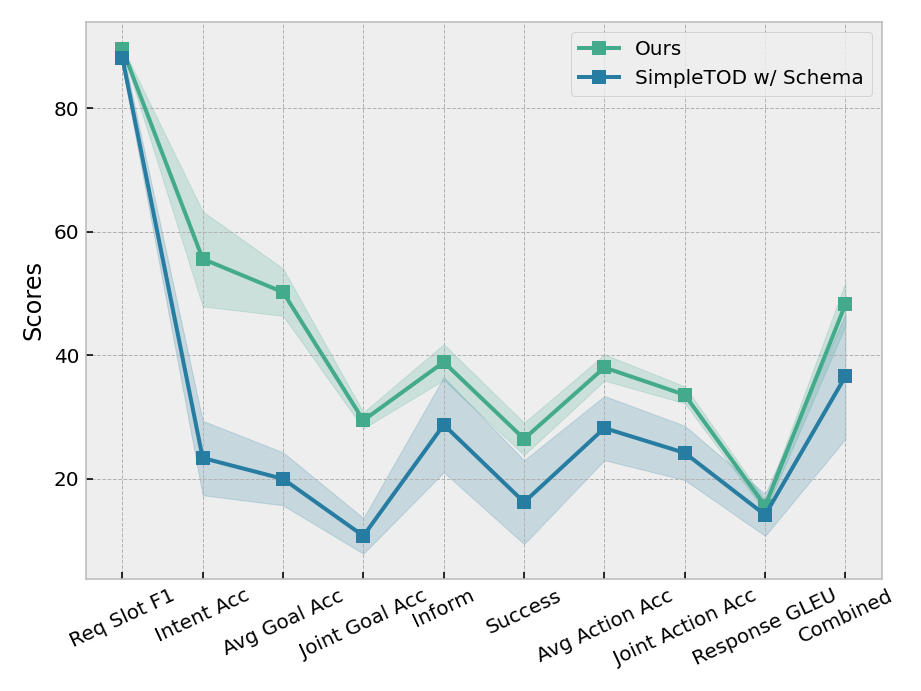
\includegraphics[width=\linewidth]{assets/sgdx_results.png}
    \caption{
        SGD-X results: For the 5 versions of SGD-X, we plot the mean of each metric and represent the standard deviation as the shaded area.
    }
    \label{fig:sgdx_graph}
\end{figure}



To access the robustness of~\oursys, we ran experiments on the unseen domains of the SGD-X dataset and the results are presented in Figure~\ref{fig:sgdx_graph}.
The line graph shows the mean of each metric across all 5 versions of SGD-X and the shaded area represents the standard deviation.
At first glance, we can see that the baseline has a much larger standard deviation than~\oursys~and upon a closer inspection, we can see that
there is more variation in metrics that evaluate the system actions: Inform, Success, AAA and JAA.
For~\oursys, we can see DST metrics have a larger standard deviation, which could be due to the fact that~\oursys~has a low Intent Accuracy metric
than other DST models as shown already in Table~\ref{tab:other-results}. \textbf{Is this too negative? Should I drop this?}




